%% IMPORTANT: Once working, run latex 3 times to get listoffigures to work

%% Be sure to check spelling!

%% Put **your** name and the proper due date in place

%% Copy the lstlisting and figure code as many times as you need
%% Be sure to put in your own file names if appropriate

\documentclass{article}
\usepackage{amsmath}    % loads AMS-Math package
\usepackage{epsfig}     % allows PostScript files
\usepackage{listings}   % allows lstlisting environment
\usepackage{moreverb}   % allows listinginput environment
\usepackage[letterpaper, margin=0.75in]{geometry}  % set paper size/margins
\usepackage[table]{xcolor}

\begin{document}
\begin{center}
\rule{6.5in}{0.5mm}\\~\\
\textbf{\large EGR 103L -- Fall 2017}\\~\\
\textbf{\huge Graphics and Loops}\\~\\
Ian Hanus (ih52)\\
Lab Section 1B, Tuesday 8:30-11:20\\
22 October 2017\\~\\
{\small I understand and have adhered to all the tenets of the Duke
  Community Standard in completing every part of this assignment.  I
  understand that a violation of any part of the Standard on any part
  of this assignment can result in failure of this assignment, failure
  of this course, and/or suspension from Duke University.} 
\rule{6.5in}{0.5mm}\\
\end{center}
\tableofcontents
\listoffigures
\pagebreak
\section{Chapra Problem 4.1}
\begin{center}
\input{DivAvgTable.tex}
\end{center}
The quality of approximations can be measured by error, or the true value minus the approximation \cite[p.~101]{Chapra}. The quality of the approximations are dependent on the factor that stopped the loop from continuing. If the stopping tolerance limited the number of iterations that the program went through, then the error of the approximations were within that stopping error. Therefore, if stopping error was the limiting factor, the times the loop was run with a smaller stopping error are more accurate. If the limiting factor was the number of iterations, the greater the number of iterations the closer the approximation will get to the real value. The size of the number that is being approximated is also a factor. The approximations of the larger numbers generally tend to have larger errors.
\section{Palm Figure 6.1-2}
Replication of figure 6.1-2 in Palm \cite[p.~265]{Palm}
\section{Palm Problems 5.33}
The temperature at the corner $x = y = 0$ is $1.47^o$C
\section{Palm Problem 4.28}
\begin{center}
\begin{tabular}{c c c c}
 & \textbf{\textit{x} location} & \textbf{\textit{y} location} & \textbf{Volume}\\
\textbf{Customer} & \textbf{(mi)} & \textbf{(mi)} & \textbf{(tons/week)}\\ \hline
1 & 10 & -10 & 6\\
2 & -11 & -13 & 2\\
3 & -8 & -17 & 5\\
4 & 27 & -26 & 2\\
5 & -3 & 14 & 6\\
6 & 16 & 5 & 9\\
7 & -26 & 22 & 7\\
8 & 14 & -8 & 7\\
9 & -17 & -21 & 3\\
10 & 25 & 4 & 4\\ \hline
\end{tabular}
\end{center}
The best location for the distribution center is at coordinate (8,-2) for a total cost of 4.9605e+02 dollars.

\pagebreak
\appendix
\section{Codes}
% Put the name of your file in the subsection name 
% and the listinginput input
% Be sure to include the community standard in codes!
% Add \clearpage commands if they make sense
% Make as many copies as you need

\subsection{RunDivAvg.m}
\listinginput[1]{1}{RunDivAvg.m}
\clearpage

\subsection{DivAvg.m}
\listinginput[1]{1}{DivAvg.m}
\clearpage

\subsection{PalmFigure612.m}
\listinginput[1]{1}{PalmFigure612.m}
\clearpage

\subsection{PalmProblem533.m}
\listinginput[1]{1}{PalmProblem533.m}
\clearpage

\subsection{PalmProblem428.m}
\listinginput[1]{1}{PalmProblem428.m}
\clearpage

\section{Figures}
% Be sure to remove % from elsfig when figure is ready
\begin{figure}[htb!p]
\begin{center}
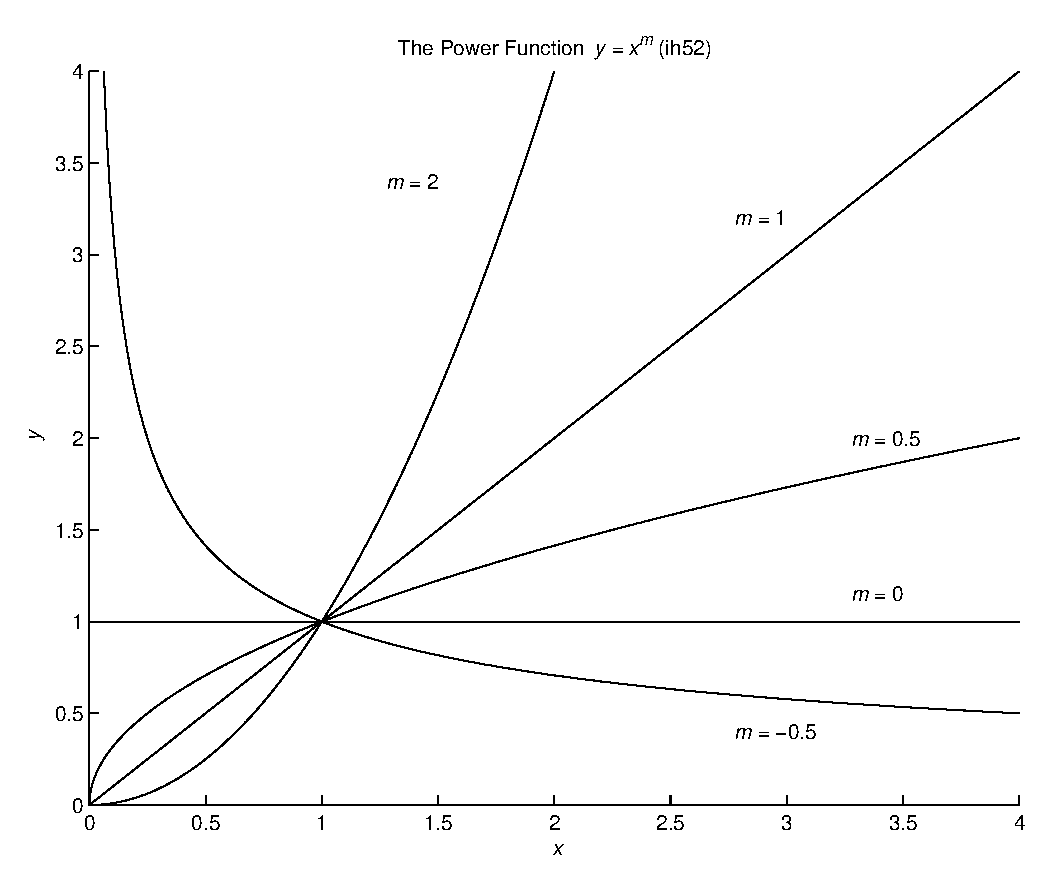
\epsfig{file=PalmFigure.eps, height=3.5in}
\caption{Palm Figure 6.1-2}
\end{center}
\end{figure}

\begin{figure}[htb!p]
\begin{center}
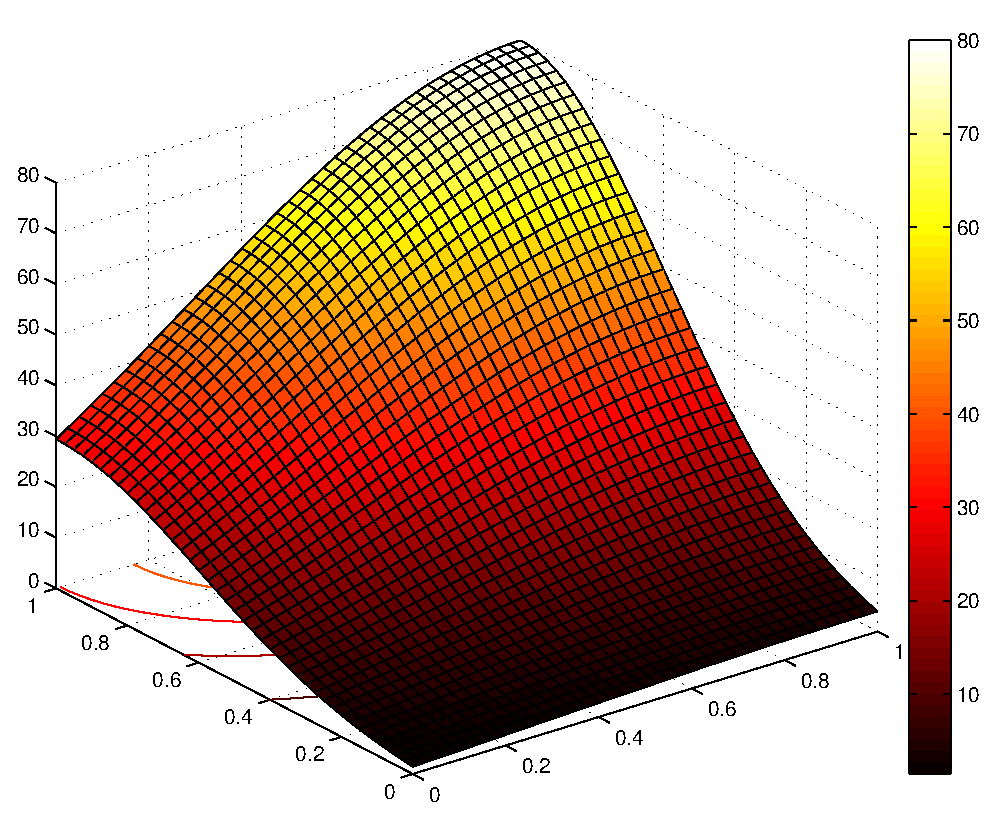
\epsfig{file=SurfacePlot533.eps, height=3.5in}
\caption{Surface Plot of Palm Problem 5.33}
\end{center}
\end{figure}

\begin{figure}[htb!p]
\begin{center}
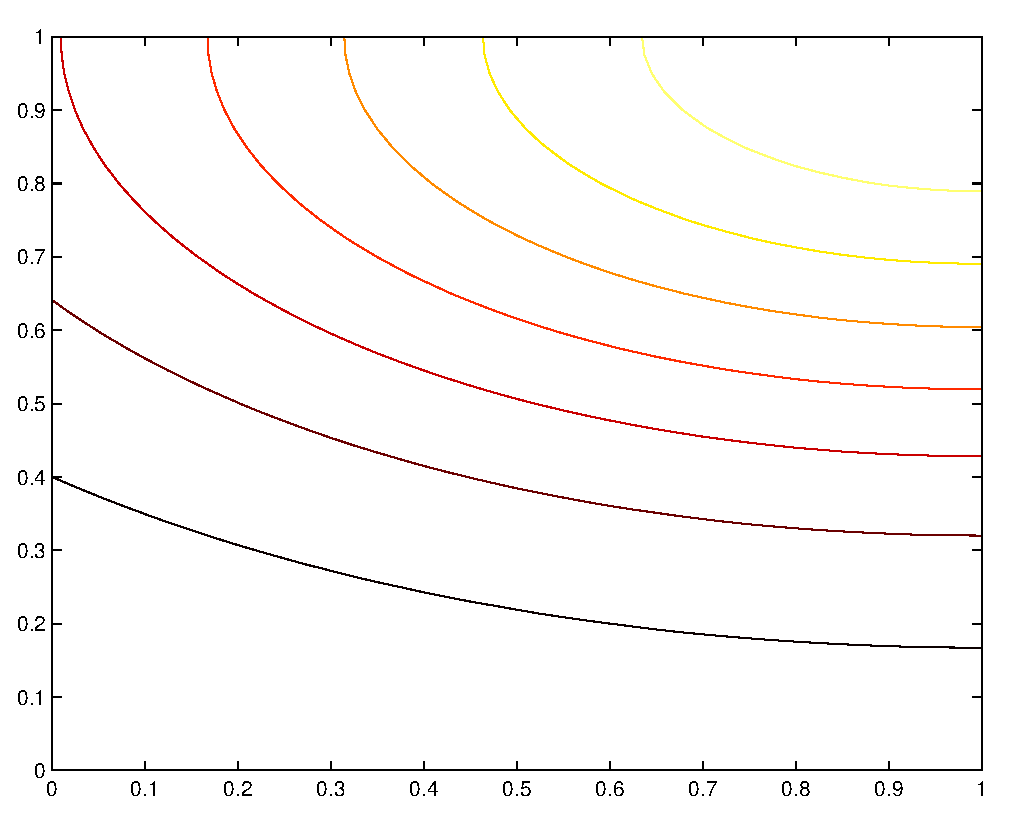
\epsfig{file=ContourPlot533.eps, height=3.5in}
\caption{Contour Plot of Palm 5.33}
\end{center}
\end{figure}

\begin{figure}[htb!p]
\begin{center}
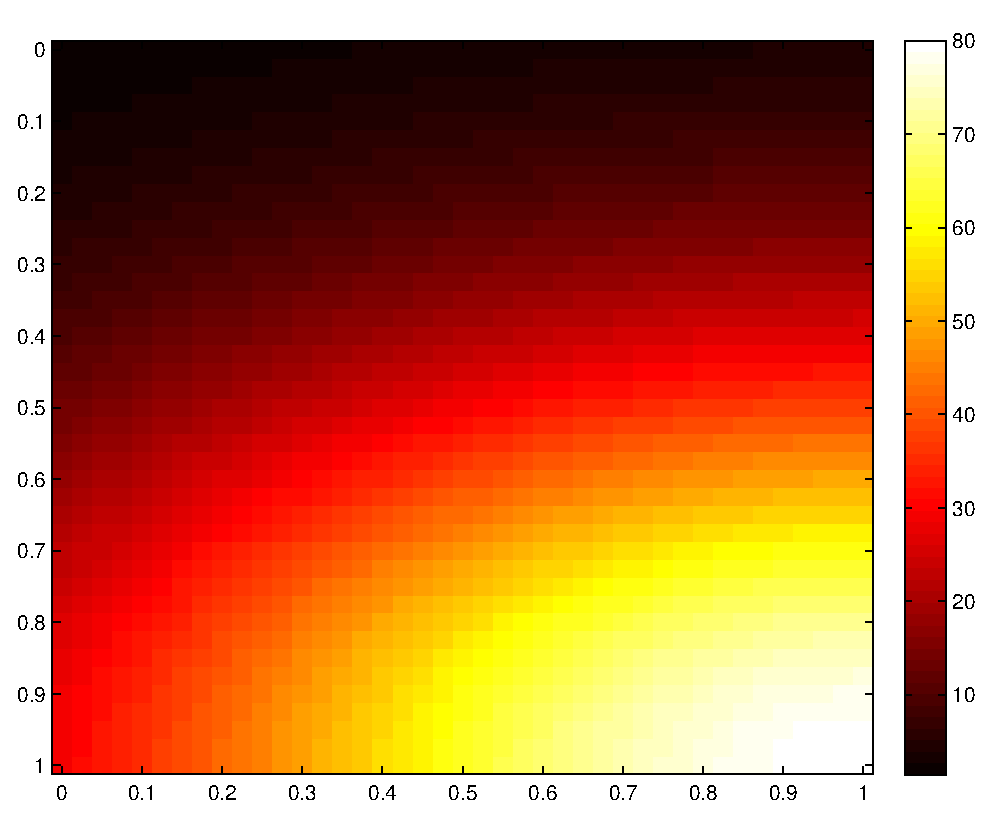
\epsfig{file=ImagescPlot533.eps, height=3.5in}
\caption{Imagesc Plot of Palm 5.33}
\end{center}
\end{figure}

\begin{figure}[htb!p]
\begin{center}
\epsfig{file=CustomerMap428.eps, height=3.5in}
\caption{Customer Map of Palm 4.28}
\end{center}
\end{figure}

\begin{figure}[htb!p]
\begin{center}
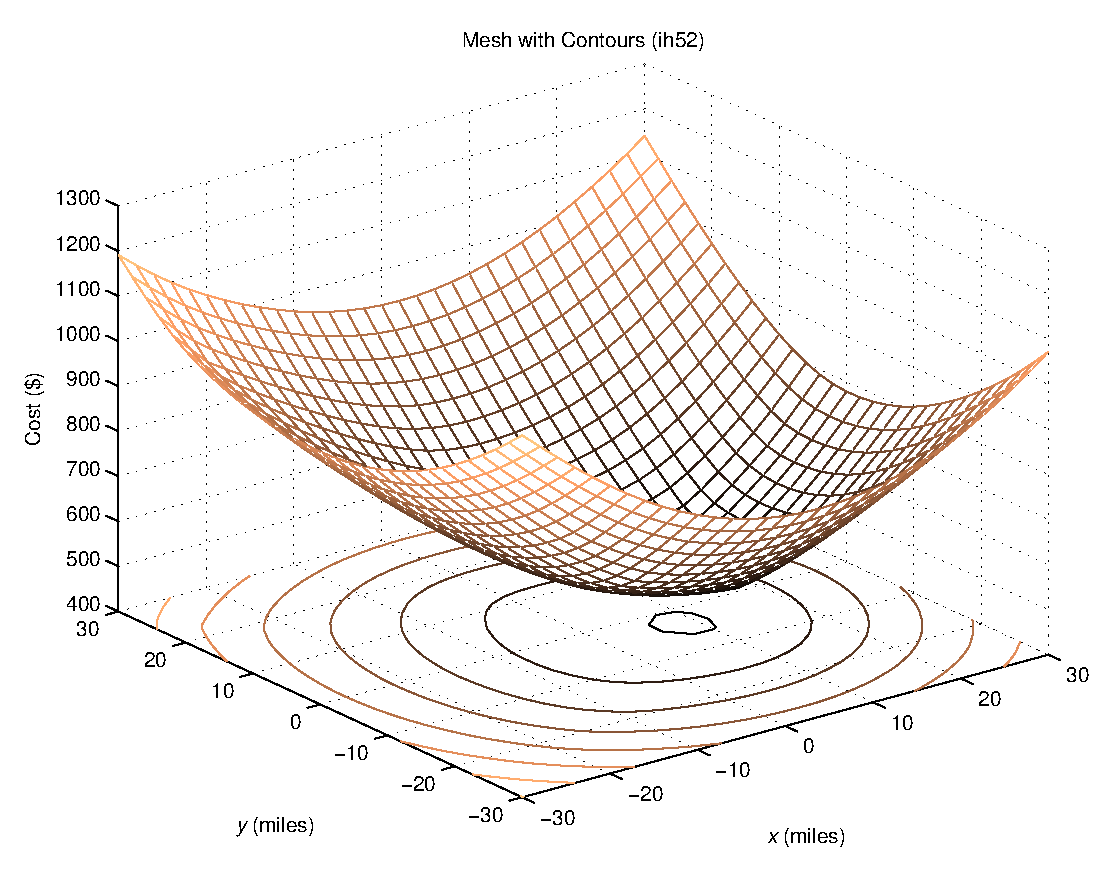
\epsfig{file=MeshContours428.eps, height=3.5in}
\caption{Mesh with Contours Plot of Palm 4.28}
\end{center}
\end{figure}

\begin{figure}[htb!p]
\begin{center}
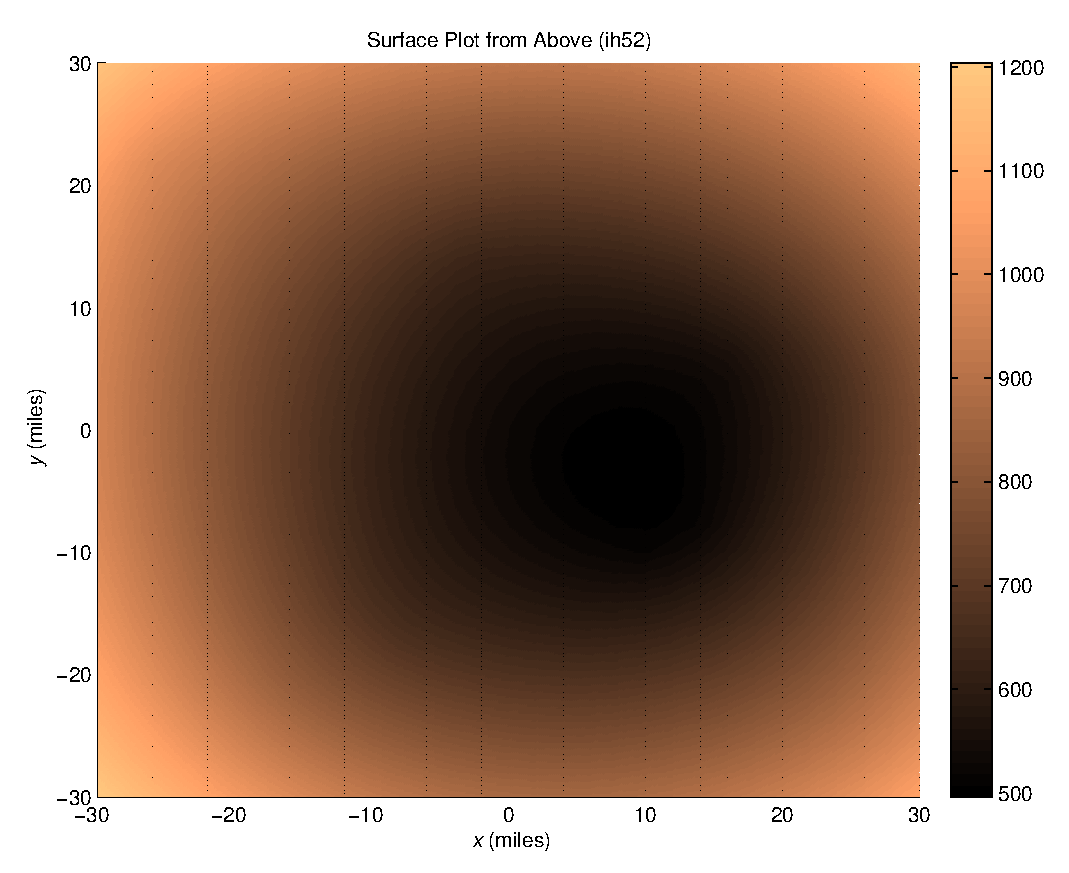
\epsfig{file=SurfacePlot428.eps, height=3.5in}
\caption{Surface Plot from Above of Palm 4.28}
\end{center}
\end{figure}

\begin{figure}[htb!p]
\begin{center}
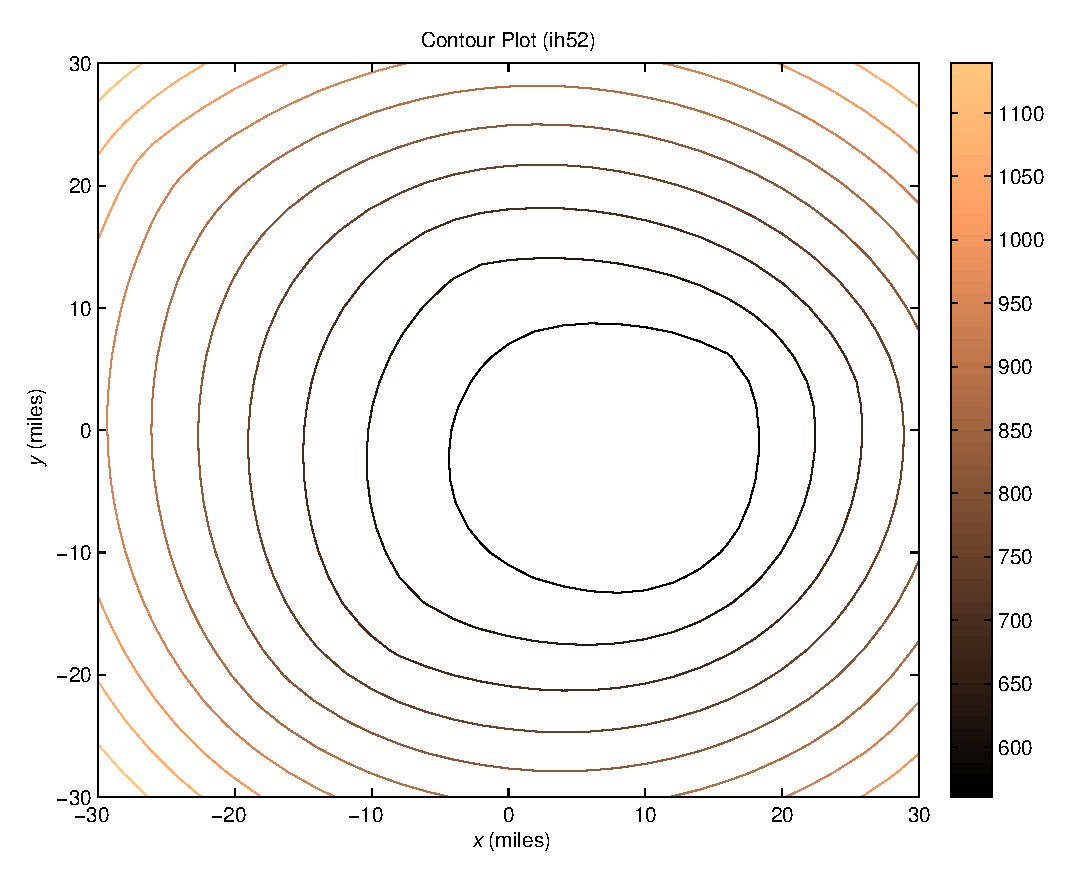
\epsfig{file=ContourPlot428.eps, height=3.5in}
\caption{Contour Plot of Palm 4.28}
\end{center}
\end{figure}
\clearpage

\begin{thebibliography}{9}
\bibitem{Chapra}
  Chapra, Steven C.,
  {\it Applied Numerical Methods with MATLAB for Engineering and Scientists}.
  McGraw-Hill, New York,
  4th Edition,
  2018.
\bibitem{Palm}
  Palm, William J.,
  {\it Introduction to MATLAB for Engineers}.
  McGraw-Hill, New York,
  3rd Edition,
  2011.
\end{thebibliography}
\end{document}
